\documentclass[12pt]{article}
\usepackage{graphicx}
\usepackage{hyperref}
\usepackage{geometry}
\usepackage{longtable}
\usepackage{float}
\usepackage{tikz}

\geometry{a4paper, margin=1in}

\title{Software Design Specification \\ \large Real-Time Safety Monitoring System for Industrial Workplaces}
\author{Syed Ahad Ali, Asad Ullah Chaudhry, Muhammad Arsalan Hussain, \\ Muzzammil Kamran Sattar}
\date{\today}

\begin{document}

\maketitle
\tableofcontents
\newpage

\section{Introduction}
This document outlines the Software Design Specification (SDS) for the Real-Time Safety Monitoring System designed for Dawlence’s sheet metal plant in Karachi. It expands upon the system requirements specified in the SRS document, focusing on the architecture, data model, pipeline, and technical implementation.

\section{Project Architecture (30 Points)}
\subsection{System Overview}
The system comprises the following major components:
\begin{itemize}
    \item \textbf{CCTV Cameras:} Capture real-time footage across factory zones.
    \item \textbf{YOLO Models:} Process video frames for safety hazard detection.
    \item \textbf{Backend Server:} Coordinates communication between system components and manages data storage.
    \item \textbf{Web-Based Dashboard:} Visualizes hazard notifications and safety analytics.
    \item \textbf{Notification System:} Delivers alerts via dashboard, email, and SMS.
\end{itemize}

% \subsection{System Block Diagram}
% \begin{figure}[h]
%     \centering
%     \includegraphics[width=\textwidth]{architecture_diagram_placeholder.png}
%     \caption{Directed System Block Diagram}
%     \label{fig:architecture}
% \end{figure}

\subsection{Design Principles}
\begin{itemize}
    \item Modular and scalable architecture to support future industrial expansions.
    \item Real-time processing with minimal latency for critical alerts.
    \item Robust security and data privacy measures.
\end{itemize}

\newpage
\section{Data Model (25 Points)}
\subsection{Database Design}
The system database manages:
\begin{itemize}
    \item \textbf{Hazard Events:} Records details such as timestamp, camera location, hazard type, and alert status.
    \item \textbf{User Data:} Stores user roles and permissions for secure system access.
    \item \textbf{Video Metadata:} Tracks file locations and annotations for incident playback.
\end{itemize}

% \subsection{Entity-Relationship Diagram}
% \begin{figure}[h]
%     \centering
%     \includegraphics[width=\textwidth]{er_diagram_placeholder.png}
%     \caption{Entity-Relationship Diagram for Data Management}
%     \label{fig:er_diagram}
% \end{figure}

\subsection{Data Annotations}
Annotated data includes:
\begin{itemize}
    \item PPE compliance (e.g., gloves, shoes).
    \item Hazard zones and restricted area boundaries.
    \item Forklift proximity and speed.
\end{itemize}

\section{Data Pipeline}
\subsection{Training Data Pipeline}
\begin{figure}[H]
    \centering
    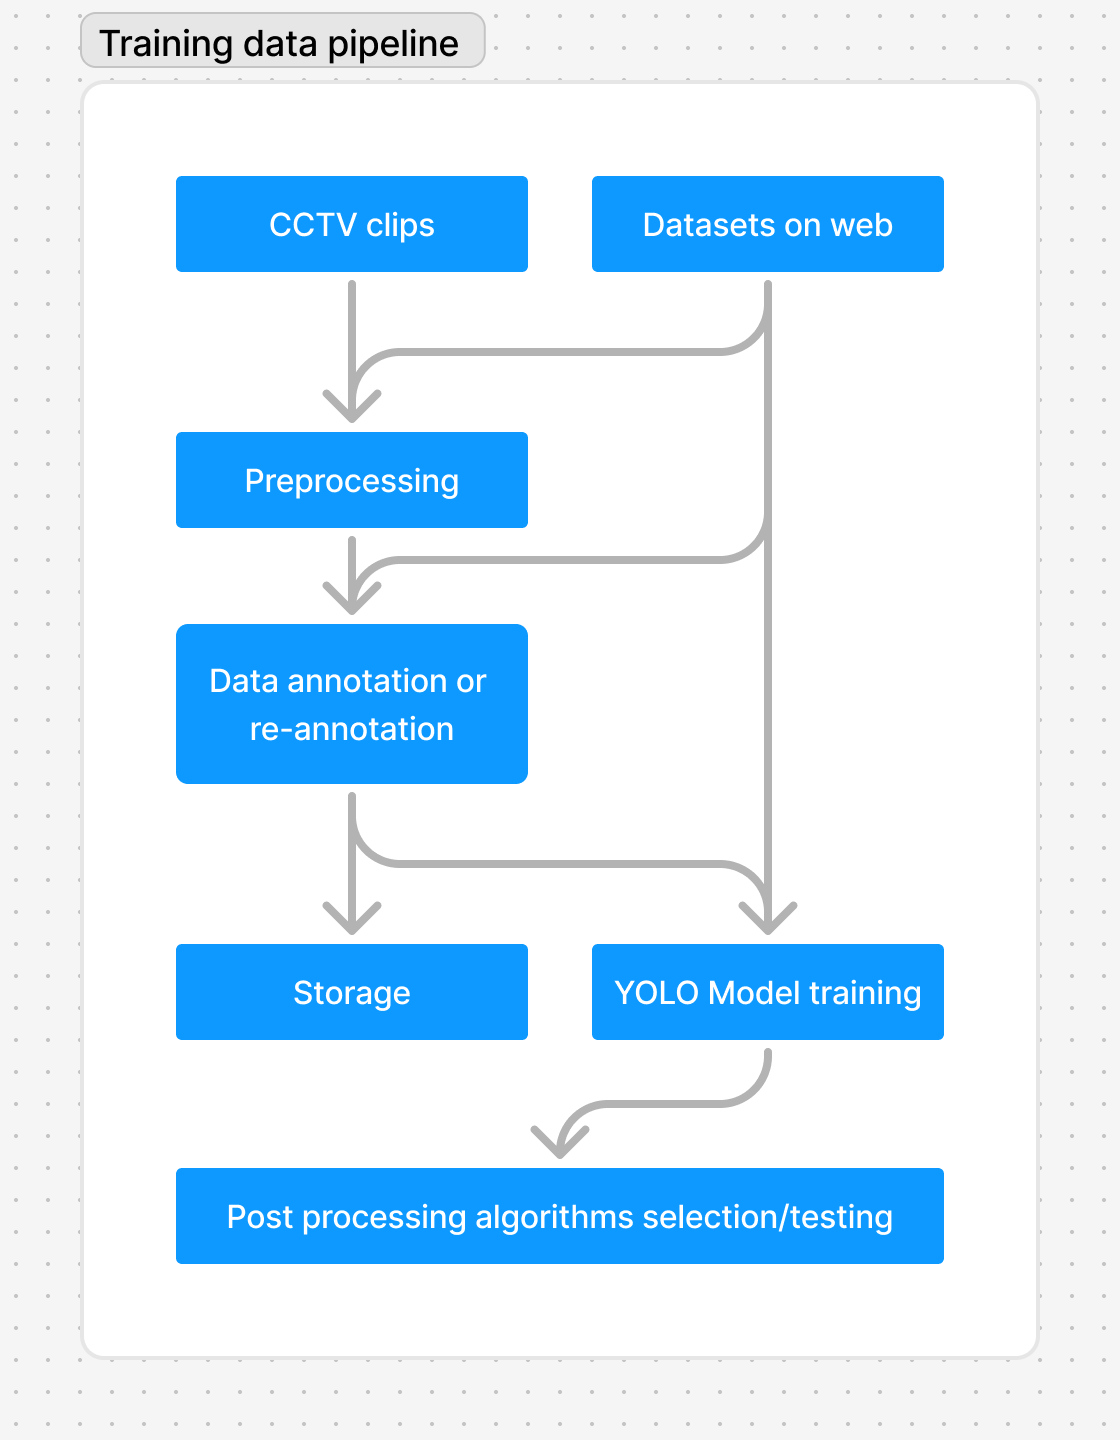
\includegraphics[width=0.75\textwidth]{training_pipeline.png}
    \caption{Training data pipeline diagram}
    \label{fig:pipeline1}
\end{figure}

\begin{enumerate}
    \item \textbf{Data Collection:} CCTV footage and publicly available datasets. Publicly available datasets may need to be preprocessed and/or re-annotated.
    \item \textbf{Preprocessing:} Frame extraction, resizing, and augmentation.
    \item \textbf{Data annotation:} Annotate frames manually.
    \item \textbf{YOLO Model Training:} Transfer learning on annotated datasets.    
    \item \textbf{Post-Processing algorithms testing:} Contextual filtering to detect hazards based on relationship of detecteions. Experiment with different methods to find most accurate for our purpose.
    \item \textbf{Storage:} Privately stored recording of CCTV clips, annotated frames and associated data.
\end{enumerate}

\subsection{Live Data Pipeline}
\begin{figure}[H]
    \centering
    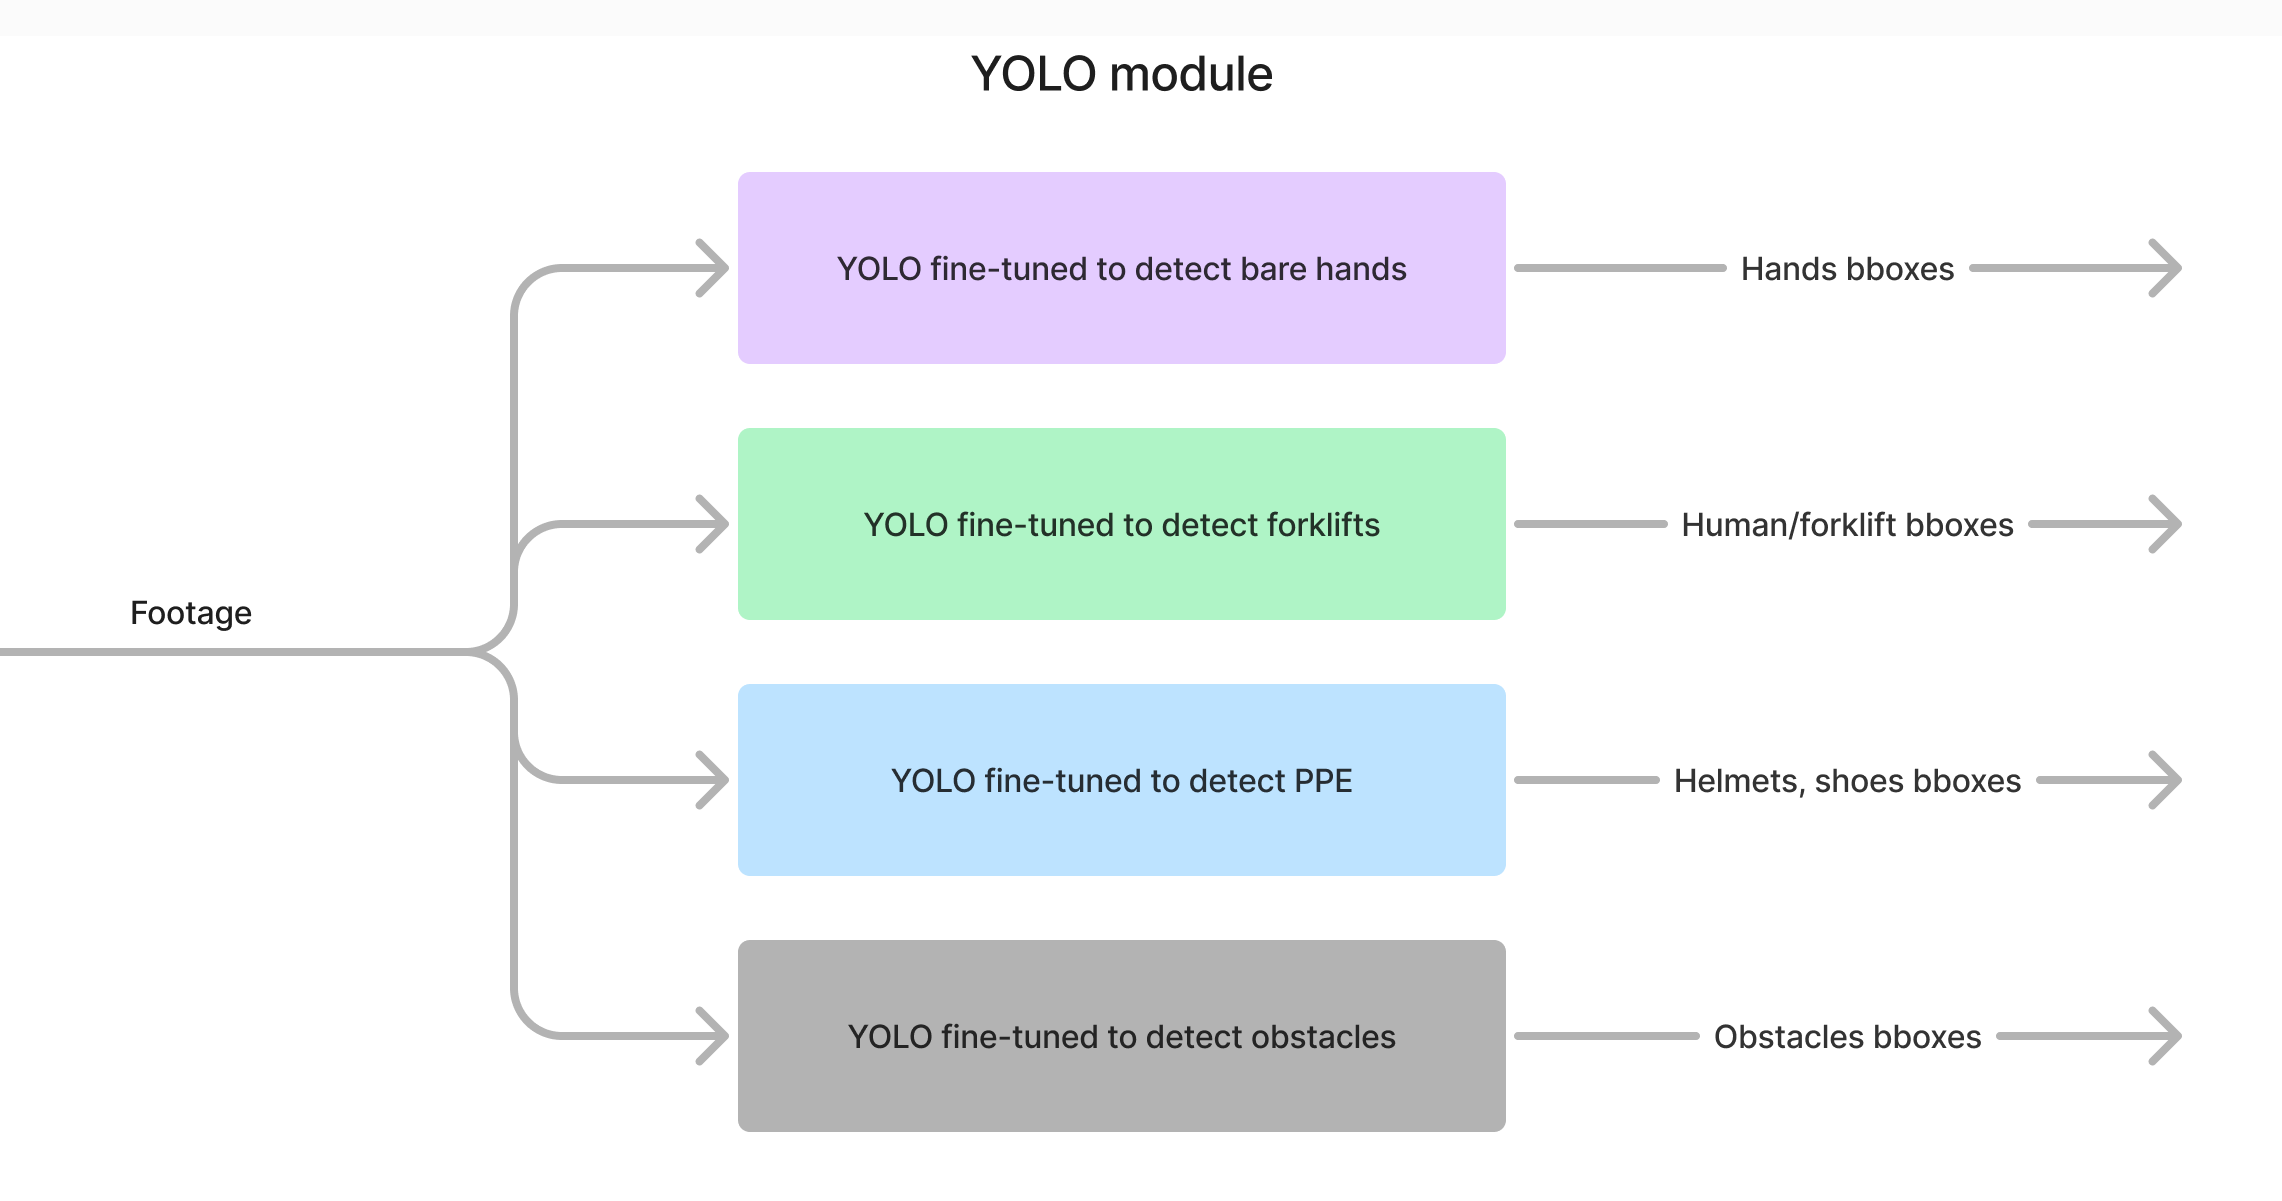
\includegraphics[width=\textwidth]{yolo_module.png}
    \caption{YOLO module: $\leq4$ YOLO models running in parallel}
    \label{fig:yolo}
\end{figure}

\begin{figure}[H]
    \centering
    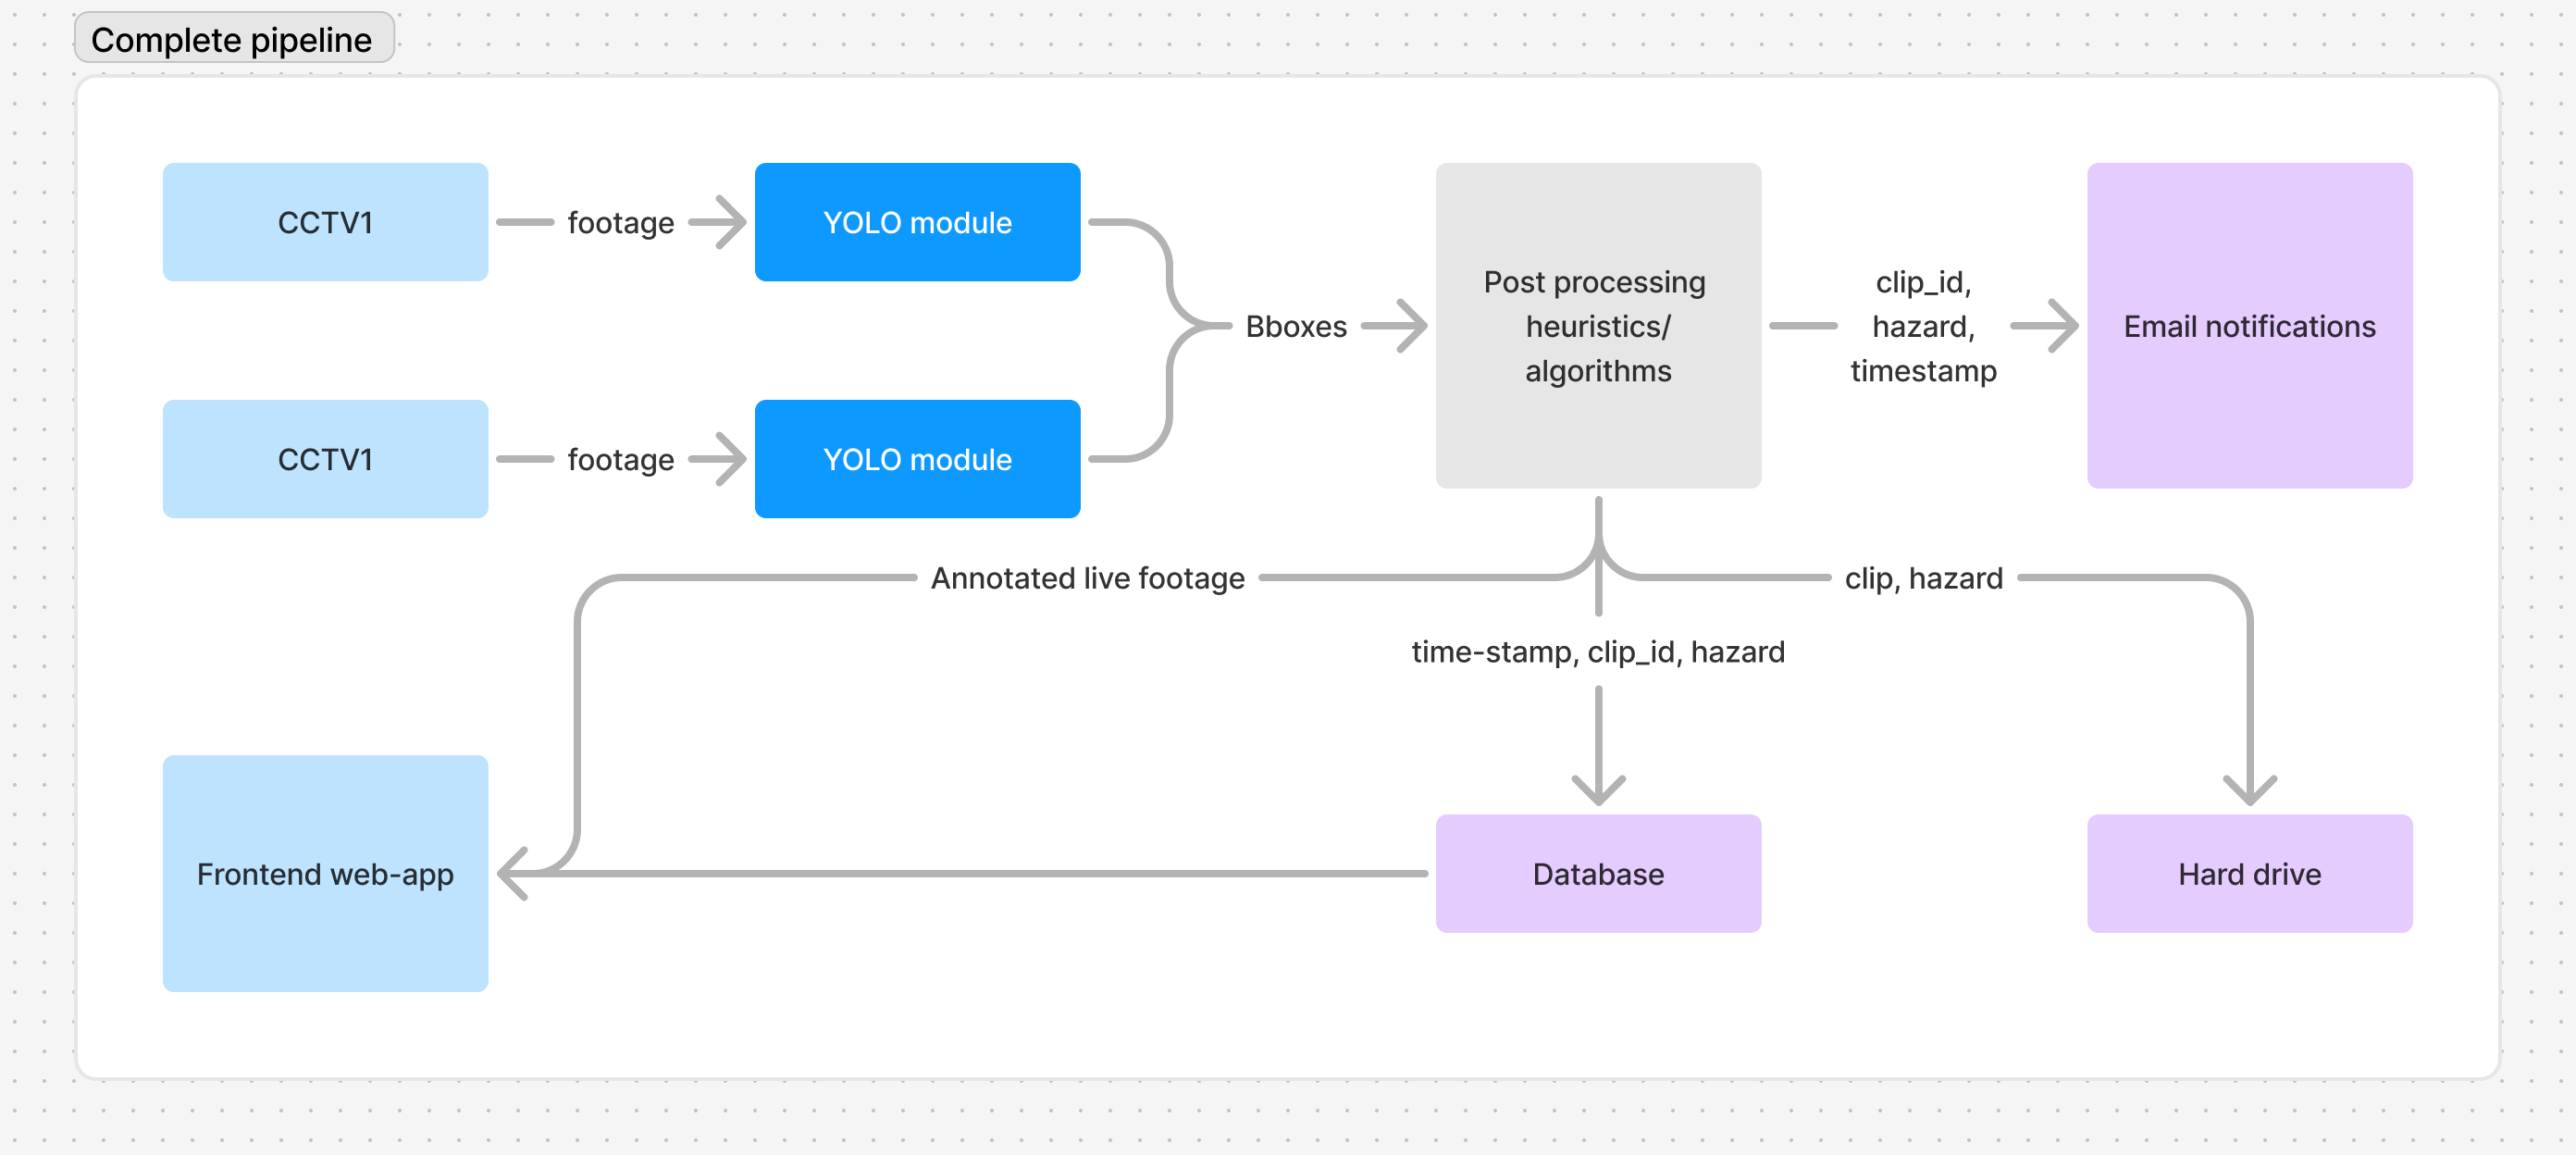
\includegraphics[width=\textwidth]{complete_pipeline.png}
    \caption{Live Data pipeline diagram}
    \label{fig:pipeline2}
\end{figure}

\begin{enumerate}
    \item \textbf{CCTV cameras}: Live video stream from CCTV cameras.
    \item \textbf{YOLO module}: $\leq$4 YOLO models running in parallel, each finetuned for a detection of safety-relevant objects.
    \item \textbf{Post Processing}: Heuristic and non-heuristic algorithms to recognize hazards via relationships of detected objects.
    \item \textbf{Database}: Relational database for statistics and records.
    \item \textbf{Hard drive}: Clips stored locally on server machine.
    \item \textbf{Frontend Web App}: An admin dashboard to look at annotated camera footage and statistics.
\end{enumerate}

\section{Technical Details (20 Points)}
\subsection{Tools and Technologies}
\begin{itemize}
    \item \textbf{Deep Learning Framework:} PyTorch.
    \item \textbf{Model:} YOLOv8 for object detection.
    \item \textbf{Frontend:} ReactJS.
    \item \textbf{Backend:} Django and MSSQL.
    \item \textbf{Notification Channels:} Email (SMTP), SMS (Twilio API).
\end{itemize}

\subsection{Performance Metrics}
\begin{itemize}
    \item Latency: Maximum of 5 seconds for hazard detection and alert delivery.
    \item Accuracy: 85\% minimum detection rate under standard conditions.
    \item Frame Rate: Processing at least 5 frames per second.
\end{itemize}

\subsection{Security Features}
\begin{itemize}
    \item Encrypted communication between components.
    \item Role-based access controls for user management.
    \item Multi-factor authentication for dashboard login.
\end{itemize}

\newpage
\section{Conclusion}
The Real-Time Safety Monitoring System integrates advanced AI models with real-time processing capabilities to ensure workplace safety. This SDS serves as a comprehensive guide for system implementation, addressing architecture, data management, processing pipelines, and technical requirements.

\end{document}
